\begin{figure}[h]
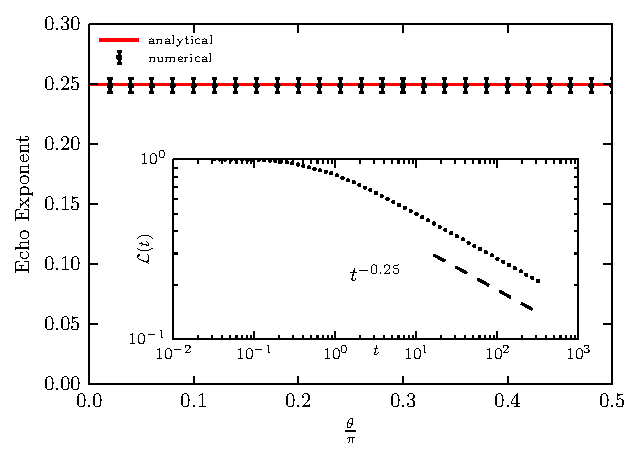
\includegraphics[width=1\columnwidth]{DDDD_fit.pdf}
\caption{The slope of the free energy for Loschmidt echo in the process $\text{DD}+\text{DD}\rightarrow\lambda+\text{DD}$, with gluing condition $S_1(\theta)$ where $\theta\in(0,\frac{\pi}{2})$. We work with total system size $N=30k$ sites, with parameters $m=10^{-8}$, $k=1$. The lattice constant is set to unity. The blue dots are the numerical results and the red line is the analytical result. As predicted, the slopes are equal for different values of $\theta$. Inset: An example of Loschmidt echo with $\theta=0.02\pi$ shown in log scale. The dashline denotes the power law with $t^{-0.25}$. The finite size effect will set in after $t=10^{3}$. The curve fitting method is described in the main text.}
\label{fig:DDDD}
\end{figure}

In order to check our analytic results, we reconsider the lattice model introduced in Sec.~\ref{sec_sub:free_boson_lattice}. In particular, we calculate the Loschmidt echo and bipartite fidelity for various joining boundary conditions determined by $S_1(\theta)$ or $S_2(\theta)$. Similar numerical evaluations exist in the literatures\cite{vasseur_universal_2014,stephan_local_2011},  however we shall follow a different approach, and the reader is referred to App.~\ref{app:comp_fid_echo} for the technical details. 

We start with the process $\text{DD}+\text{DD}\rightarrow\lambda+\text{DD}$ and the numerical simulation is performed for $\theta=0.02n\pi$, $n=1,...,25$. The results for Loschmidt echo is shown in Fig.~\ref{fig:DDDD}, and numerical parameters are given in the caption. The green dots correspond to numerical results for the slope of free energy, and the solid line shows the analytical result for echo in Eq.~\eqref{eq:result_DDDD}. The inset shows the double logarithmic plot of Loschmidt echo versus time for the case $\theta=0.02\pi$. The dashline denotes the expected power law decay $\mathcal{L}(t)\sim t^{-0.25}$. For the curve fitting, we randomly pick a data point near $t=10$ and fit the lower half of the data. This is repeated five times and we calculate the mean and standard deviation for the exponents. With the data processing method described, the error bar in the main figure is invisible on the data points. We have performed the identical simulation for the process $\text{NN}+\text{NN}\rightarrow\lambda+\text{NN}$ and obtained identical result shown in Fig.~\ref{fig:DDDD} (the initial decay of Loschmidt is different but has the same exponent at larger time). We note one caveat for this case with Neumann boundary conditions on both sides of the chain. Because of the zero mode, it is expected (indeed we saw) that the numerical simulation may not be stable. The problem can be avoided by adding a small mass regulator $m=10^{-8}$. We have performed similar numerical analysis to calculate the free energy for fidelity, and it matches the result in Eq.~\eqref{eq:result_DDDD}. We shall not show the result here. 

Next we analyze the process $\text{DN}+\text{DN}\rightarrow\lambda+\text{DN}$ in which the joining boundary condition is determined by $S_1(\theta)$. There is one subtly which is that $S_1(0)$ corresponds to `DN' and the process reduces to $\text{DN}+\text{DN}\rightarrow\text{DN}+\text{DN}$. The zero mode will cause the numerical simulation unstable near $\theta=0$, and it turns out that the mass regulator cannot resolve this problem. Rather, we shall shift one of the `DN' slightly and consider the following process
\begin{eqnarray}\begin{aligned}
\label{eq:approx_DNDN}
S_1(0)+S_1(\delta\theta)\rightarrow S_1(\theta)+S_1(\delta\theta)
\end{aligned}\end{eqnarray}
where we take $\delta\theta=0.003\pi$ and $\theta=0.02n\pi$, $n=1,...,25$. In the limit $\delta\theta=0$, Eq.~\eqref{eq:approx_DNDN} reduces to the process we would like to study. The issue of extra bcc at $-\infty$ due to $\delta\theta$ will be discussed in Sec.~\ref{sec:disc}. We show the numerical result for Loschmidt echo in Fig.~\ref{fig:DDNN}(a). The slope of the free energy follows a quadratic relation as predicted in Eq.~\eqref{eq:result_DNDN}. The deviation from the analytic result (without the shift) near $\theta=0$ has been greatly suppressed because of $\delta\theta$ introduced manually. The cost is that the numerical results near $\theta=0.5\pi$ was shifted slightly, which will match more precisely if $\delta\theta=0$. We demonstrated the $\theta$-dependence of power law in the inset. To confirm that zero mode is responsible for the unexpected behavior near $\theta=0$, we numerically calculate the free energy for fidelity, which is immune to the zero mode. The simulation is performed in the same setup with  $\delta\theta=0.001\pi$. The result is shown in Fig.~\ref{fig:DDNN}(b), which shows perfect match between numerical and analytical results. 

Further we consider the case $\text{P}+\text{P}\rightarrow\lambda+\text{P}$, and the numerical results for Loschmidt echo and fidelity are shown in Fig.~\ref{fig:PPPP}(a). Since $S_2(\frac{\pi}{4})$ corresponds to periodic boundary condition, numerical instability will set in near $\theta=\frac{\pi}{4}$ due to the zero mode. We shift one of the periodic boundary condition slightly 
\begin{eqnarray}\begin{aligned}
\label{eq:approx_DNDN}
S_2\left(\frac{\pi}{4}\right)+S_2\left(\frac{\pi}{4}+\delta\theta\right)\rightarrow S_2(\theta)+S_2\left(\frac{\pi}{4}+\delta\theta\right)
\end{aligned}\end{eqnarray}
where we take $\delta\theta=0.003\pi$ and $\theta=0.02n\pi$, $n=1,...,25$. 
\todo[inline]{Describe the result for PP}
As a diagnostic tool, the result for fidelity is presented in Fig.~\ref{fig:PPPP}(b). 

\begin{figure}
  \centering
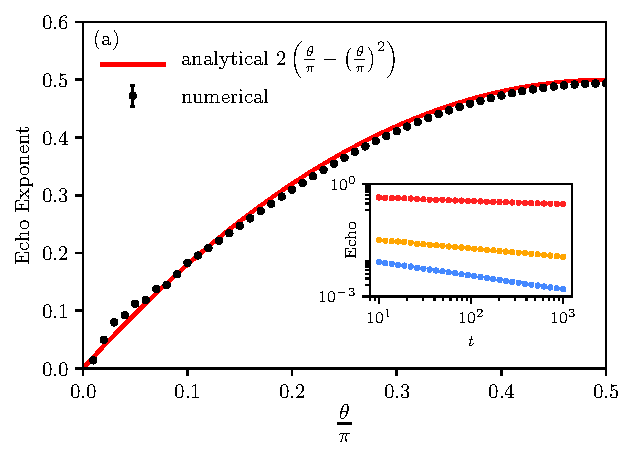
\includegraphics[width=1\columnwidth]{DDNN_fit.pdf}
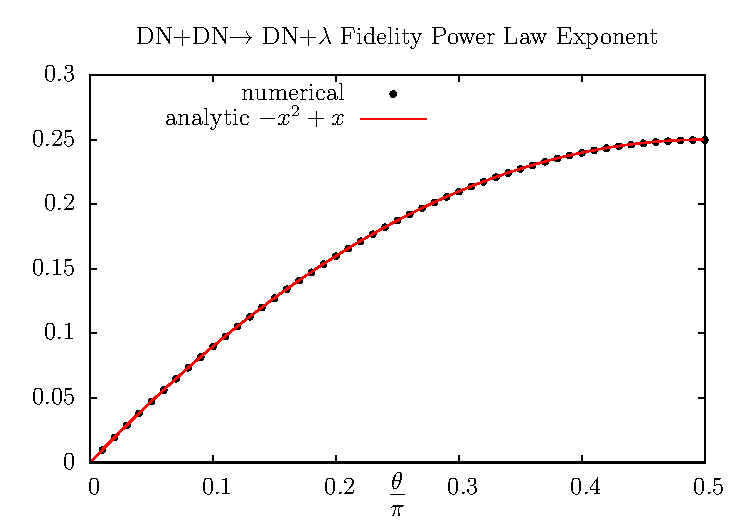
\includegraphics[width=1\columnwidth]{DN_DN2tan.pdf}
    \caption{The slope of the free energy for Loschmidt echo (a) and bipartite fidelity (b) in the process $\text{DN}+\text{DN}\rightarrow\lambda+\text{DN}$. The total system size is $N=35k$ sites with the same parameters in Fig.~\ref{fig:DDDD}. The numerical value of slopes follow a quadratic relation as predicted. For the deviation from the analytic results in (a), see the discussion in the main text. Inset in (a): From the top to bottom, we show the power law decay of Loschmidt echo with $\theta=0.02\pi, 0.12\pi,0.24\pi$ and $0.48\pi$. The finite size effect will set in after $t=10^{4}$. We use the same curve fitting method as described for Fig.~\ref{fig:DDDD}.}
      \label{fig:DDNN}
    \todo[inline]{Tianci: make the plots have the same style?}
\end{figure}


\begin{figure}
  \centering
  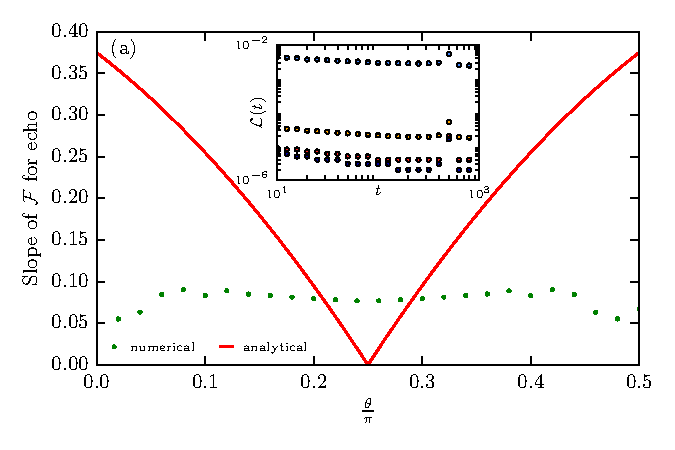
\includegraphics[width=1\columnwidth]{PP_fit.pdf}
    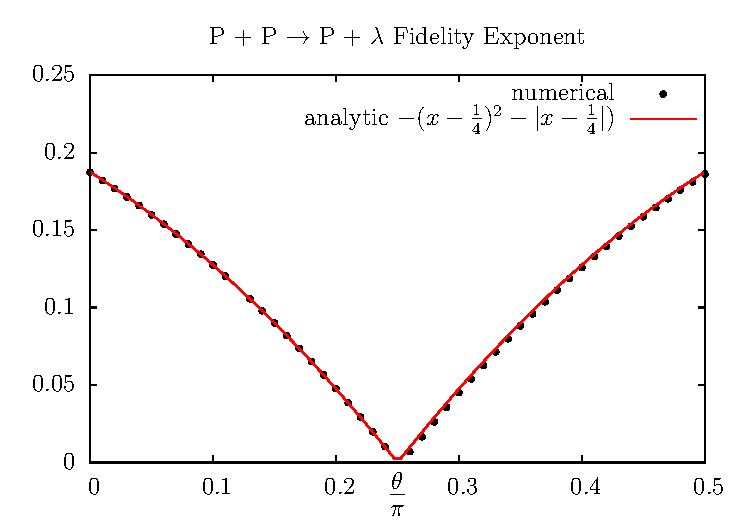
\includegraphics[width=1\columnwidth]{p_p2tan.pdf}
    \caption{The slope of the free energy for Loschmidt echo (a) and bipartite fidelity (b) in the process $\text{P}+\text{P}\rightarrow\lambda+\text{P}$. The parameters are the same as those in Fig.~\ref{fig:DDNN}. The plot is symmetric with respect to $\theta=0.25\pi$ as predicted. For the deviation from the analytic results in (a), see the discussion in the main text. Inset in (a): From the top to bottom, we show the power law decay of Loschmidt echo with $\theta=0.02\pi, 0.12\pi,0.24\pi$ and $0.48\pi$. The finite size effect will set in after $t=10^{4}$. We use the same curve fitting method as described for Fig.~\ref{fig:DDDD}.}
    \label{fig:PPPP}
    \todo[inline]{Mao: Put the PPPP for echo; Tianci: make the plots have the same style?}
\end{figure}

